\section{Introduction}

Drivers enter a parking lot without having any specific knowledge about the
lot's availability. Especially in urban areas, it is common for any driver to
spend an additional, non-trivial amount of time looking for a parking spot. This
searching time not only translates into frustration but also wastes energy and
produces carbon dioxide harmful for the environment.

In order to assist drivers searching for a parking space, numerous smartphone
applications are developed and available in the online application stores.
Although many drivers find these smartphone applications useful, these
applications either do not provide real-time parking lot availability or
just displays publicly-accessible availability information. 

To overcome this limitation, a few academic systems have been
proposed~\cite{4212497, Chen:2012:COS, Delot:2009:CRP, 5062057,
Mathur:2010:PDS}. However, these systems make a variety of assumptions that
prevent them from being immediately deployable. Typical assumptions include, the
availability of additional infrastructure~\cite{5062057}, additional equipment
deployed on vehicles~\cite{Mathur:2010:PDS}, the presence of a vehicular
network~\cite{Delot:2009:CRP, Mathur:2010:PDS, 4212497}, and manual inputs from
users~\cite{Chen:2012:COS}.

We present {\it PocketParker}, a system that predicts parking lot availability
using smartphones. Unlike previous approaches, our goal is to not require any
additional input or infrastructure other than the smartphones used by the users
of PocketParker. In order to accomplish this goal, we address two main
challenges. We accomplish this goal by combining an activity detector
deployed as a smartphone appplication that automatically extracts park and
depark events as well as a prediction model that estimates parking lot
availability based on observed events. Our activity detector addresses the
challenges of energy efficiency and accuracy of detection. Our prediction model
addresses the challenges of estimating the number of {\it hidden drivers} who do
not participate in PocketParker as well as arrival and departure rates of a
parking lot. Using this information, PocketParker probabilistically estimates
how many parking spots are available at any given time.

\begin{figure}
\centering
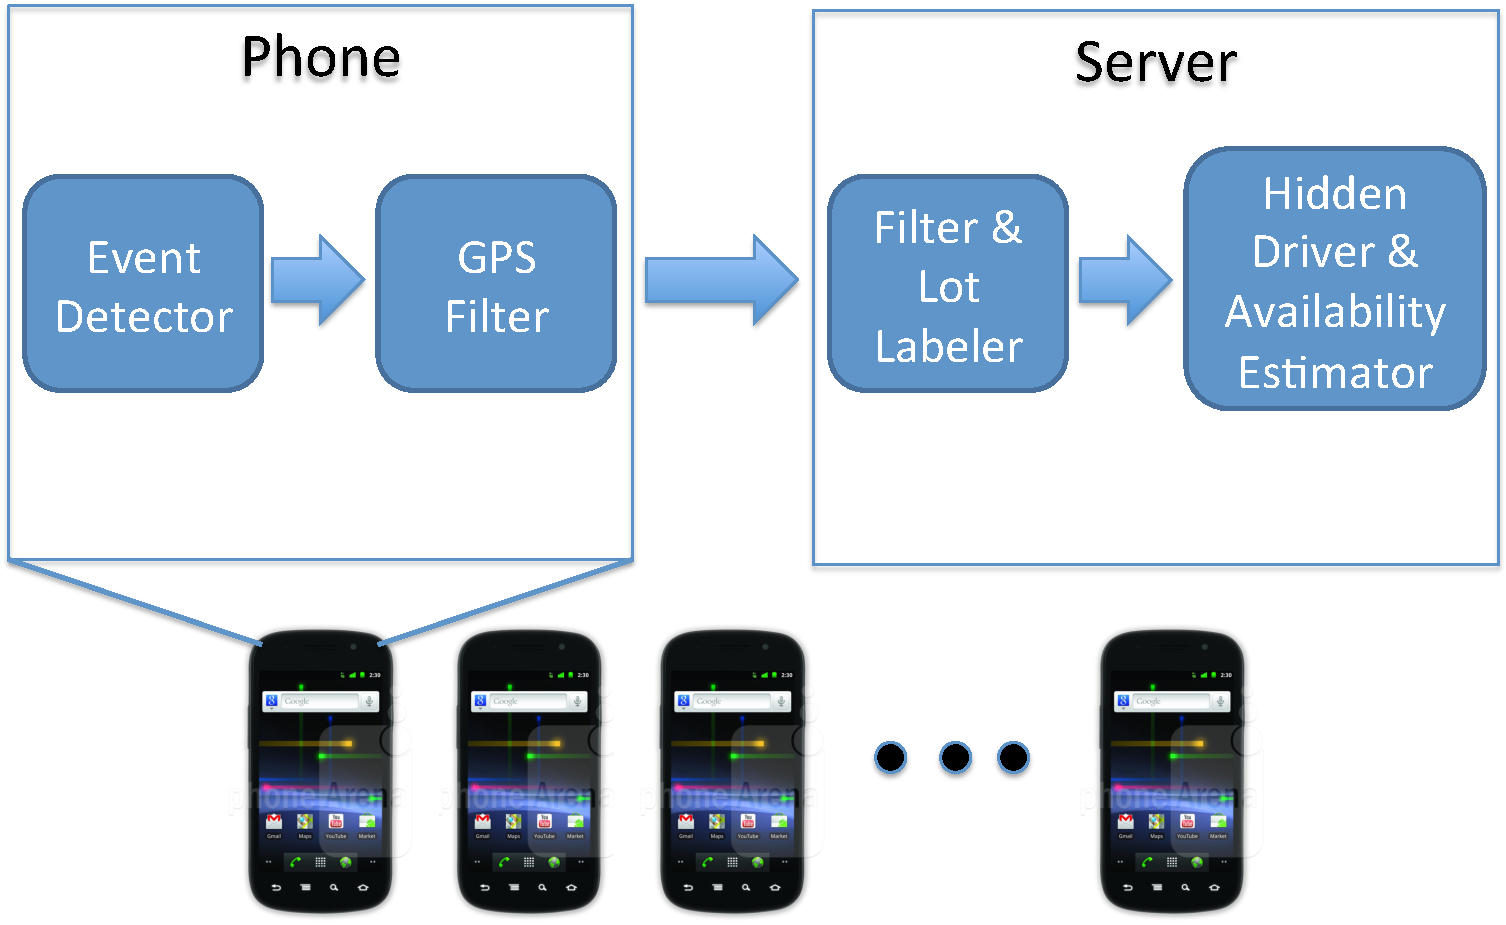
\includegraphics[width=\columnwidth]{./figures/blockdiagram.pdf}

\caption{\textbf{PocketParker architecture.}}

\label{fig-arch}
\end{figure}

\subsection{Usage Model}
